\section{Módulo de Sistemas Inteligentes}

{\justify
    \hspace{0.5cm} Para el módulo de sistemas inteligentes se utilizó un
    \textbf{Perceptrón Multicapa} para la clasificación de color utilizando el sensor
    \textbf{TCS230} para esto, la red tiene 3 nodos de entrada para realizar la
    clasificación y fue entrenada con 600 muestras diferentes de colores.

    \hspace{0.5cm} Para comenzar, primero veremos el proceso básico utilizado para el
    \textbf{Perceptrón Simple}

}

\subsection{El Perceptrón Simple}
\begin{center}
    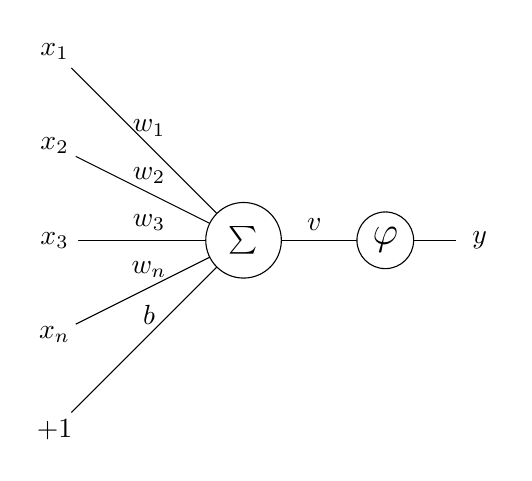
\begin{tikzpicture}[scale=0.6]
        \draw (0,4) -- node[above]{$w_1$} (4,0);
        \draw (0,2) -- node[above]{$w_2$} (4,0);
        \draw (0,0) -- node[above]{$w_3$} (4,0);
        \draw (0,-2) -- node[above]{$w_n$} (4,0);
        \draw (0,-4) -- node[above]{$b$} (4,0);
        \draw (4,0) -- node[above]{$v$} (7,0);
        \draw (7,0) -- (9,0);

        \foreach \i in {4,2,...,-4}{\fill[white] (0,\i) circle (5mm);}
        \fill[white] (9,0) circle (5mm);

        \node at (0,4){$x_1$};
        \node at (0,2){$x_2$};
        \node at (0,0){$x_3$};
        \node at (0,-2){$x_n$};
        \node at (0,-4){$+1$};
        \node at (9,0){$y$};

        \draw[color=black,fill=white] (4,0) circle (8mm);
        \node at (4,0){\Large $\sum$};

        \draw[color=black,fill=white] (7,0) circle (6mm);
        \node at (7,0){\Large $\varphi$};
    \end{tikzpicture}
\end{center}

{\justify
    \hspace{0.5cm} Primero de tiene la ecuación en la que interactuan los patrones de
    entrada con los pesos sinápticos y el \textbf{bias}, que se puede representar de
    diferentes formas, como

    \begin{equation}
        v = \sum_{i=1}^p [w_i x_i] + b
    \end{equation}

    \begin{equation}
        v =
        \begin{bmatrix}
            w_1 & w_2 & \cdots & w_p
        \end{bmatrix}
        \begin{bmatrix}
            x_1 \\
            x_2 \\
            \vdots \\
            x_p
        \end{bmatrix} + b
    \end{equation}

    \begin{equation}
        v = w^\top x + b
    \end{equation}

    \hspace{0.5cm} El valor $v$ de esta ecuación se pasa por una función $\phi(v)$ para
    obtener la salida del \textbf{Perceptrón}, que queda representada como

    \begin{equation}
        y = \varphi(v)
    \end{equation}

    \hspace{0.5cm} Después, se obtiene un error con

    \begin{equation}
        e = d - y
    \end{equation}

    \hspace{0.5cm} En dónde $d$ es el valor deseado para el patrón de entrada y $y$ el
    valor obtenido por el perceptrón. Con el valor de $e$ obtenido, se ajustan los pesos
    sinápticos y bias de la siguiente forma

    \begin{align}
        w &\leftarrow w + \eta e x \\
        b &\leftarrow b + \eta e
    \end{align}

    \hspace{0.5cm} En donde $\eta$ es el factor de aprendizaje del perceptrón.
    Con esto, se tiene completado el proceso de aprendizaje del
    \textbf{Perceptrón Simple}. Ahora conociendo esto, podemos avanzar con las ecuaciones
    y el proceso de aprendizaje del \textbf{Perceptrón Mutlicacpa}

}

\subsection{El Perceptrón Multicapa}

\begin{center}
    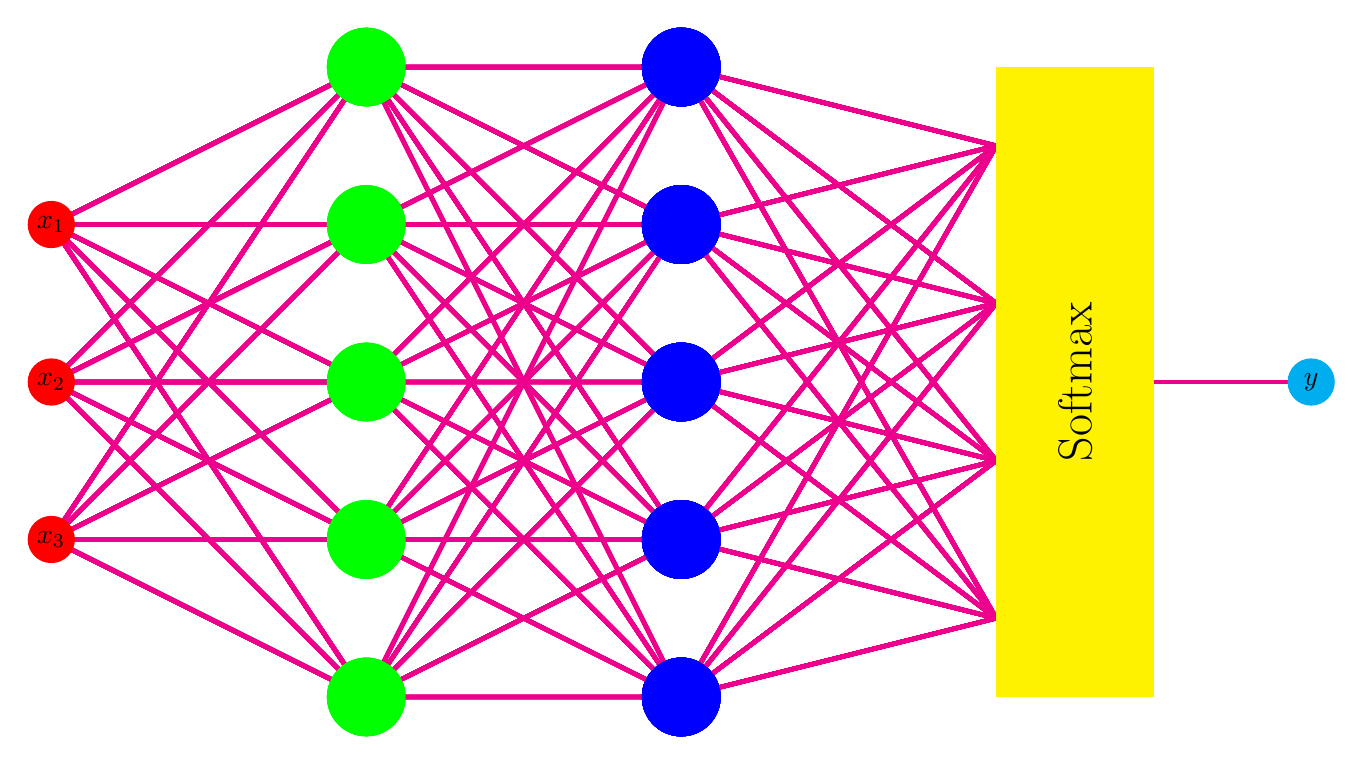
\begin{tikzpicture}
        \foreach \a in {2,0,-2}{
            \foreach \b in {4,2,...,-4} {
                \foreach \c in {4,2,...,-4}{
                    \foreach \d in {3,1,-1,-3}{
                        \draw[color=magenta, ultra thick] (0,\a)--(4,\b)--(8,\c)--(12,\d);

                    }

                    \fill[blue] (8,\c) circle (5mm);
                }

                \fill[green] (4,\b) circle (5mm);
            }

            \fill[red] (0,\a) circle (3mm);
        }
        \draw[color=magenta, ultra thick] (14,0)--(16,0);
        \fill[cyan] (16,0) circle (3mm);
        \node at (16,0){$y$};

        \node at (0,2){$x_1$};
        \node at (0,0){$x_2$};
        \node at (0,-2){$x_3$};

        \fill[yellow] (12,4) rectangle (14,-4);
        \node at (13,0){\LARGE\rotatebox{90}{Softmax}};
    \end{tikzpicture}
\end{center}

{\justify
}

